\section{Introdução a Memória em C}

\subsection{Layout de Memória em C}

Uma representação típica de memória de um programa em C consiste das seguintes partes:
\begin{itemize}
  \item \textbf{Segmento de texto:} seções de um programa que contém instruções de execução;
  \item \textbf{Segmento de dados inicializados:} porção do espaço de endereço virtual que contém
    variáveis globais e estáticas que foram inicializadas pelo programador;
  \item \textbf{Segmento de dados não inicializados (BSS):} aqui ficam as variáveis globais e
    estáticas não inicializados pelo programador ou inicializados com valor 0;
  \item Heap: onde acontece a \textbf{alocação dinâmica}. Ela começa no final do segmento BSS e vai
    crescendo de tamanho. Ela é gerenciada por \textit{malloc}, \textit{realloc} e \textit{free};
  \item Stack: onde fica a \textit{stack} do programa, com política LIFO (\textit{Last In First
    Out}).Variáveis automáticas são armazenadas aqui e informações salvas a cada chamada de uma
    função. Essa parte da memória é vital para o funcionamento de recursões em C;
\end{itemize}

\begin{figure}[H]
  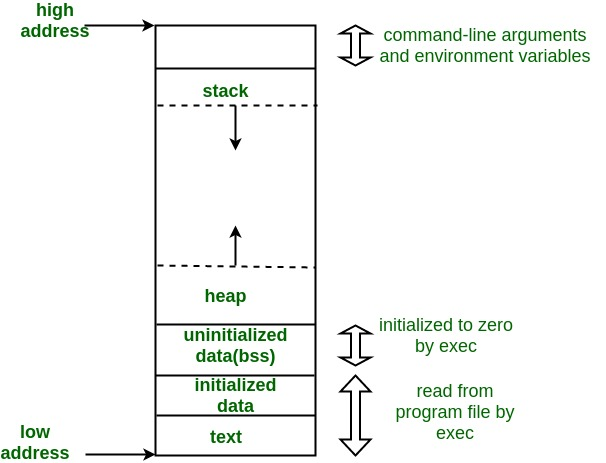
\includegraphics[scale=0.5]{assets/memory-layout-c.jpeg}
  \centering
  \caption{Layout de memória de programas em C - GeeksforGeeks}
\end{figure}

\subsection{\textit{Heap} e \textit{Stack}}

\paragraph{Heap} Na Heap, a memória é alocada durante a execução das instruções (código) escrito.
Ela é um espaço de memória disponível para desenvolvedores manipulá-la, alocando e desacolando
blocos de memória conforme necessário. Quando fazemos um objeto ele é criado na Heap e as
informações de referência são sempre armazenadas na \textbf{Stack}. Um ponto importante quando
estamos manipulando a Heap é tomar cuidado para não termos um vazamento de memória (\textit{Memory
Leak}). Por isso é importante estarmos usando a função \textit{free()}.

\paragraph{Stack} Na Stack, a alocação acontece em blocos de memória contíguos. Aqui, o tamanho de
memória a ser alocada é conhecida pelo compilador e, sempre que uma função é chamada, suas variáveis
tem sua memória alocada na \textit{Stack}. Um ponto a ressaltar aqui é que o programador não precisa
se preocupar em ficar alocando e desalocando memória explicitamente, já que todo esse processo é
responsabilidade do compilador.
\subsection{Variáveis em C}

Antes de entender como os ponteiros funcionam precisamos relembrar o conceito de variável.
Uma variável é um bloco reservado na memória para armazenar algum valor. Em C podemos definir e inicializar
uma variável da seguinte forma:

\begin{lstlisting}[language=C]
int x = 0;
\end{lstlisting}

O primeiro termo se refere ao \textit{datatype} da variável, o segundo termo se refere ao nome daquela
variável que vamos usar para acessá-la e o terceiro termo é o valor que vamos armazenar naquele bloco. Além disso, podemos acessar também o endereço de memória onde
aquele bloco foi reservado.

\begin{lstlisting}[language=C]
int x = 0;
printf("O endereco e: %d", &x);
\end{lstlisting}

O código de bloco acima realiza \textbf{alocação de memória estática}, ou seja, a alocação da memória
é feita pelo compilador e não podemos mudar seu tamanho depois de alocada.

Devemos lembrar que cada tipo de variável ocupa um espaço na memória. Por exemplo, uma variável
do tipo \textbf{int} ocupa 4 \textit{bytes}. Já uma variável do tipo \textbf{long long int} ocupa 8 \textit{bytes}.
Saber disso é importante para garantirmos que não estamos desperdiçando espaço ou que temos espaço suficiente
para o que desejamos, e será algo que vamos precisar quando formos realizar alocação dinâmica.

\subsection{Definição e Notação de Ponteiros}
Quando digitamos \textit{int x = 0;} estamos armazenando o valor 0 na variável \textit{x}. No entanto,
também podemos armazenar o \textbf{endereço} de cada variável em uma outra variável de um tipo específico:
\textbf{variável ponteiro}.

\begin{lstlisting}[language=C]
int x = 0;
int* ptrX = &x;
printf("O valor e: %d", x);
printf("O endereco e: %d", ptrX);
\end{lstlisting}

Note que temos o \textbf{*} logo depois do \textbf{int}. Ele nos diz que o tipo daquela variável é um
ponteiro para um \textbf{int}, ou seja, ela não armazena um \textbf{int} propriamente dito, mas sim o
endereço de uma variável do tipo \textbf{int}.

Além disso, note que usamos o \textit{\%d} para estarmos mostrando o endereço que aquele
ponteiro está armazenando. Isso não é totalmente correto, pois endereços de memórias devem ser mostrados
como hexadecimais. Dessa forma o mais correto seria usar o \textit{\%p} para mostrar ponteiros. No entanto,
endereços de memória também pode ser mostrando com um inteiro decimal ou como octais,
por isso o código anterior não acusa nenhum erro.

